\begin{textblock*}{\posterboxwidth * 3/4}(0pt,0pt)%
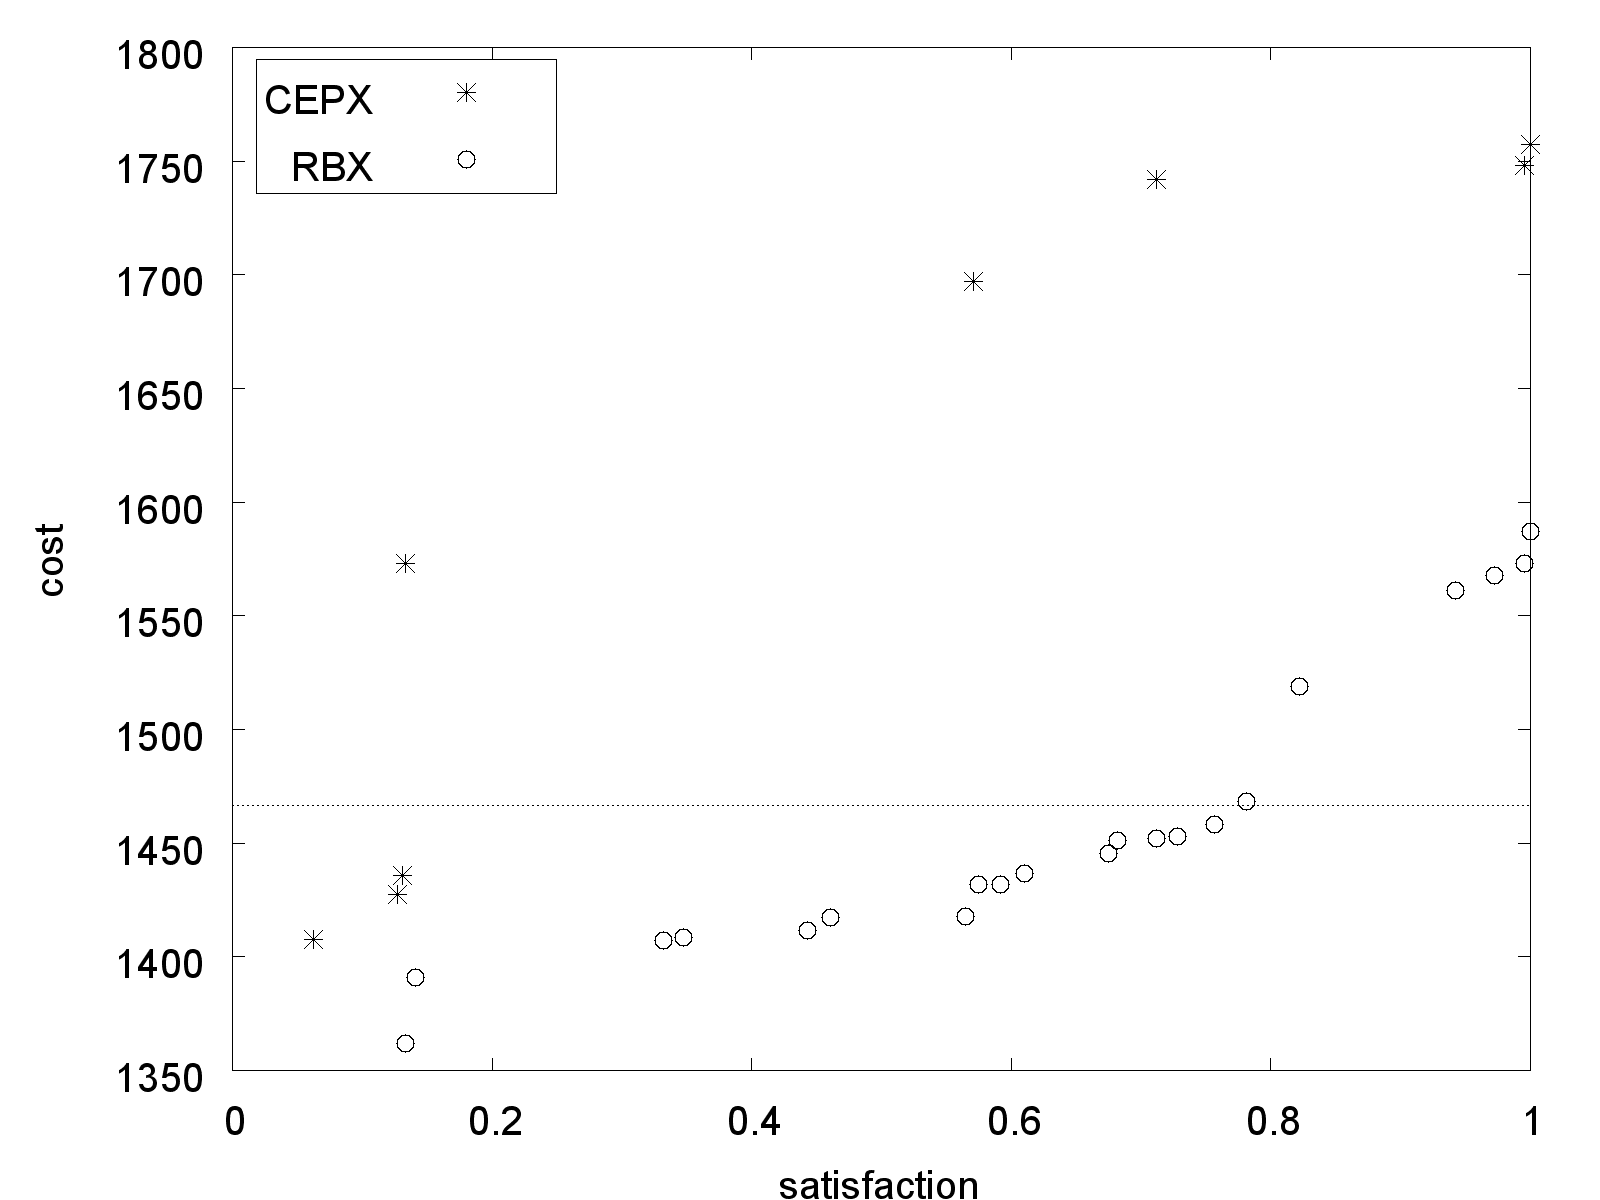
\includegraphics[width=\posterboxwidth * 3 / 8]{bitmap/R102}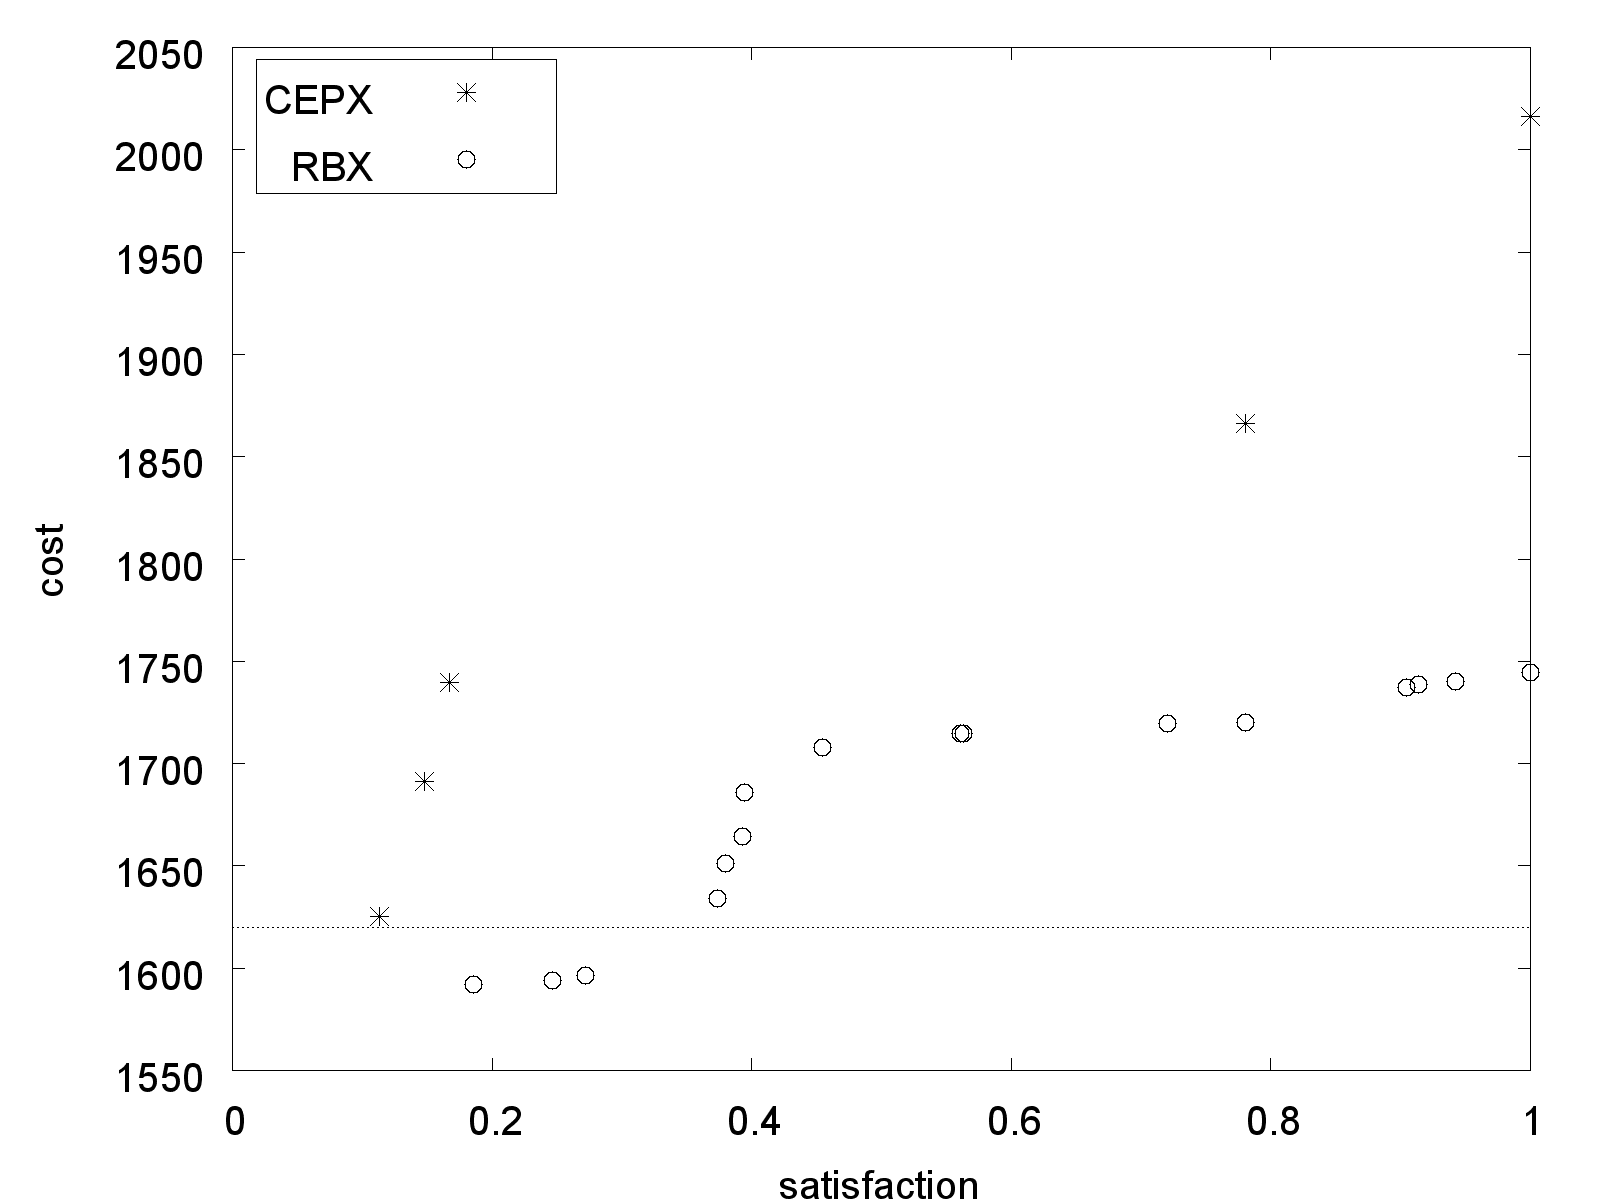
\includegraphics[width=\posterboxwidth * 3 / 8]{bitmap/RC101}%
\end{textblock*}

% komentarz tekstowy
\begin{textblock*}{\posterboxwidth / 4}(\posterboxwidth * 3 / 4, 0pt)%
\textbf{Advantages}
\begin{mylist}
\item diversified solutions
\item lower cost and satisfaction vs. high cost and satisfaction
\item possibility of choice of a solution
\item possibility of renegotiation of time windows
\end{mylist}%
\end{textblock*}

% rozwiazania ze zbioru Pareto
\newcommand\twolines[2]{\vbox{\hbox{#1}\vskip.5em\hbox{#2}}}
\begin{textblock*}{\posterboxwidth}(0pt,\posterboxheight / 3 + 3ex)%
\centering%
\textbf{Examples of solutions from a Pareto set}\\[1ex]
\begin{tabular}{ccccc}
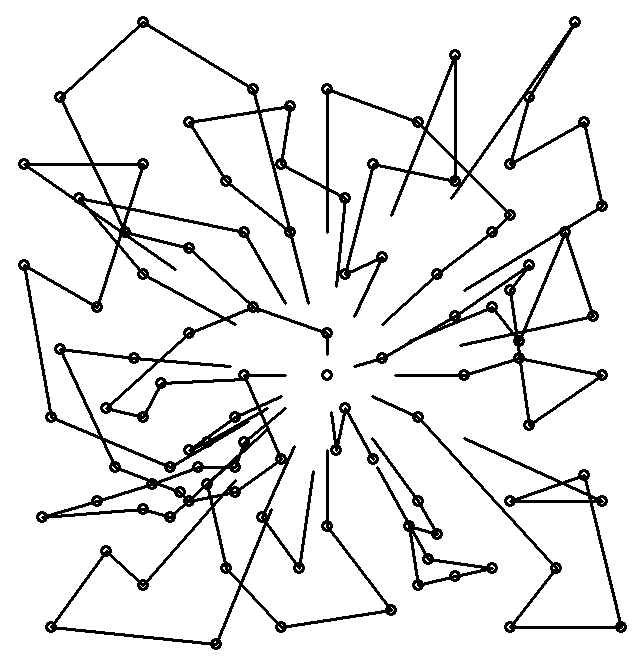
\includegraphics[height=\posterboxheight / 4]{bitmap/R102_2_Solutions_1} & \hspace{2ex} &
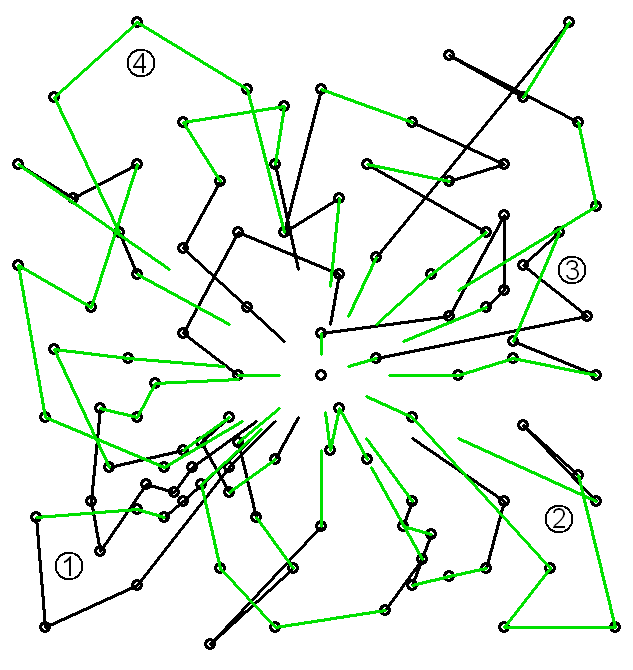
\includegraphics[height=\posterboxheight / 4]{bitmap/R102_2_Solutions_2} & \hspace{2ex} &
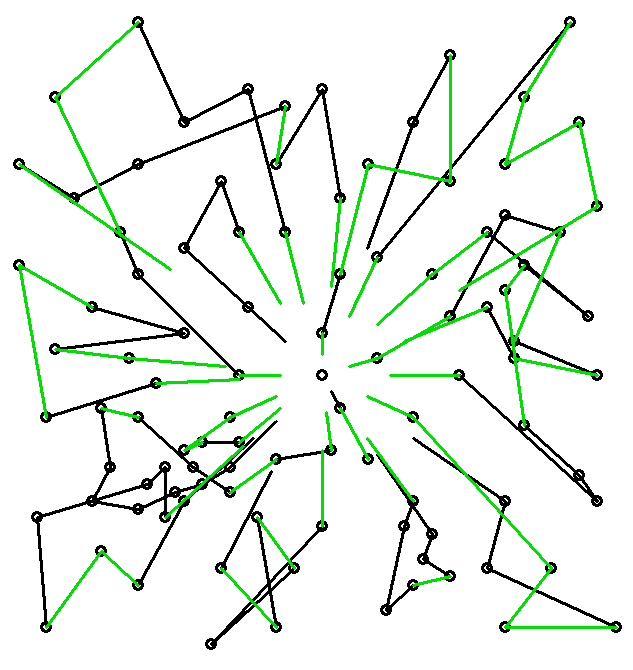
\includegraphics[height=\posterboxheight / 4]{bitmap/R102_2_Solutions_3} \\
\twolines{routes = 19}{sat = 1.0; cost = 1587} & &
\twolines{routes = 16}{sat = 0.68; cost = 1451} & &
\twolines{routes = 15}{sat = 0.13; cost = 1362}
\end{tabular}
\\[1ex]

% szczegoly rozwiazania
\centerbox{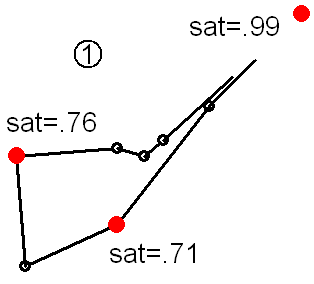
\includegraphics[scale=0.4]{bitmap/R102_2_Route1}}%
\centerbox{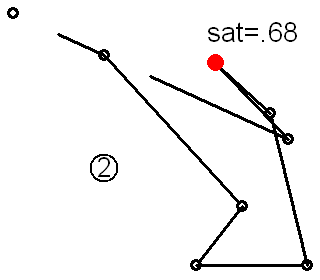
\includegraphics[scale=0.4]{bitmap/R102_2_Route2}}%
\centerbox{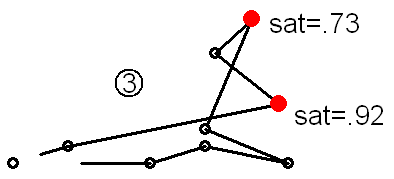
\includegraphics[scale=0.4]{bitmap/R102_2_Route3}}%
\centerbox{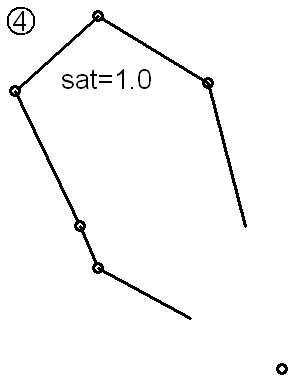
\includegraphics[scale=0.4]{bitmap/R102_2_Route4}}%
\end{textblock*}
